\documentclass[en,hazy,normal,blue,14pt]{elegantnote}

\usepackage{pgfplots}
\usepackage{caption}
\usepackage{subcaption}

\title{Notes for QF603: Quantitative Analysis of Financial Market}

\author{Zhou Shen}
\institute{Singapore Management University}

\version{1.0.0}
\date{\today}

\begin{document}
\maketitle
% logo
\centerline{\includegraphics[width=0.8\textwidth]{D:/SMU/SMU-LKCSB-logo.png}}
\newpage
\section{Session1 Introduction}
\subsection{Basic of Probability Theory}
\subsubsection{Variables}

\begin{itemize}
    \item (Discrete Random Variable)
    $\mathbb{P}(X = x_i) = p_i, i = 1,2,\cdots,n$
    \item (Continuous Random Variable)
    $\mathbb{P}(r_1<X<r_2) = p$
\end{itemize}

\subsubsection{Probability Density Functions(PDF)}
For the probability $p$ of $X$ lying between $r_1$ and $r_2$, we define the probability density function $f(x)$ as follows:
\[
    \int_{r_1}^{r_2}f(x)dx = p    
\]
\subsubsection{Cumulative Distribution Functions(CDF)}
Let f(x) be the CDF. A cumulative distribution function $F(a)$ tells us probability of a random variable $X$ being less than a certain value $a$:
\[
F(a) = \int_{-\infty}^a f(x)dx = \mathbb{P}(X\leq a)
\]

For CDF, we have following properties:
\begin{itemize}
    \item $f(x)=\frac{dF(x)}{dx}$
    \item $\mathbb{P}(a<X\leq b) = \int_a^bf(x)dx = F(b)-F(a)$
    \item $\mathbb{P}(X>a)=1-F(a)$
\end{itemize}

\subsubsection{Inverse Cumulative Distribution Functions}
Let $F(a)$ be the cumulative distribution function. We define the inverse function $F^{-1}(p)$, the inverse cumulative distribution, as follows:
\[
    F^{-1}(p) = a
\]

The inverse distribution function is also called the \textbf{quantile function}.

The inverse distribution function has following properties:

\begin{itemize}
    \item $F^{-1}(p)$ is non-decreasing.
    \item $F^{-1}(y) \leq x $ if and only if $y\leq F(x)$.
    \item If $Y$ has a uniform distribution in the interval $[0, 1]$, then $F^{-1}(Y)$ is a random variable with distribution $F$.
    \begin{remark}
    If Y has a uniform distribution in the interval $[0, 1]$, we get $F(Y) = Y$, then $F^{-1}(Y) = Y$.
    \end{remark}
\end{itemize}

\subsubsection{Mutually Exclusive Events}

For a given random variable, the probability of any of two mutually exclusive events A and B occurring is just the sum of their individual probabilities.
\[
\mathbb{P}(A\cup B) = \mathbb{P}{(A)} + \mathbb{P}{(B)}    
\]

\subsubsection{Independent Events and Joint Probability}

If the outcome of one random variable is not influenced by the outcome of the other random variable, then we say those variables are independent. The joint probability of $A$ and $B$ is such that
\[
\mathbb{P}(A\cap B) = \mathbb{P}{(A)} \mathbb{P}{(B)}    
\]

\subsubsection{Probability Matrices}
When dealing with the joint probabilities of two variables, it is often convenient to summarize the various probabilities in a probability matrix or probability table.

\begin{example}
\begin{figure}[!ht]
	\centering
	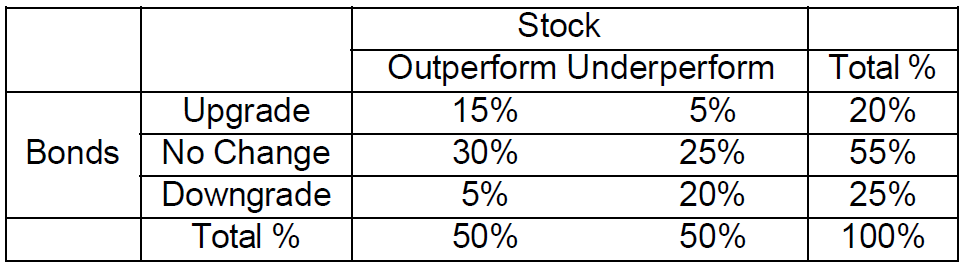
\includegraphics[width=\textwidth]{probability_matrix.png}
	\caption{Stock Grading by Equity Analyst and Credit Rating
    Agency}
\end{figure}
\end{example}

\subsubsection{Conditional Probability}
Probability of A given that B is:
\[
\mathbb{P}(A|B) = \frac{\mathbb{P}(AB)}{\mathbb{P}(B)}
\]

If $\mathbb{P}(A|B) = \mathbb{P}(A)$ , the two random variables $A$ and $B$, are independent.

\subsection{Bayesian Analysis}
\subsubsection{Definition}
For two random variables, $A$ and $B$, Bayes’ theorem states that
\[
    \mathbb{P}(A|B) = \frac{\mathbb{P}(B|A)\mathbb{P}(A)}{\mathbb{P}(B)}
\]

\begin{remark}
    To see sample problems, go for QF603session1 pdf from page45 to page68.
\end{remark}

\section{Statistics and inference}

\subsection{Basics of Statistics}
\subsubsection{Statistical Population}

Statistical population is the set of all possible elements that are of interest for a statistical analysis.
\begin{example}
    The time series of split-adjusted daily stock prices of Dell Inc. since IPO on June 22, 1988 till taken private on October 29, 2013.
\end{example}

\subsubsection{Moment Generating Function}
Let $X$ be a random variable with pdf $f(x)$. The moment generating function(mgf) of X is:
\[
    \begin{aligned}
        M_x(\theta) &= \mathbb{E}[e^{\theta x}]\\
        &= 1 + \mathbb{E}[x]\theta + \mathbb{E}[x^2]\frac{\theta^2}{2!} + \mathbb{E}[x^3]\frac{\theta^3}{3!} + \cdots
    \end{aligned}
\]

$M_x^n(0)$ gives us the $n$th moment of the distribution of the random variable $x$:
\begin{itemize}
    \item $\mu = M_x^1(0)$ 
    \item $\sigma^2 = \mathbb{E}[x^2]-(\mathbb{E}[x])^2 = M_x^2(0) - (M_x^1(0))^2$
    \item $\mathrm{Skewness} =  \mathbb{E}(x^3) - 3 \mathbb{E}(x) \mathbb{E}(x^2) +2 (\mathbb{E}(x))^3$\\
    \phantom{}\qquad \qquad \,$=   M_x^3(0) - 3(M_x^1(0))^2M_x^2(0) + 2(M_x^1(0))^3   $
    \item $\mathrm{Kurtosis} = \mathbb{E}(x^4) - 4\mathbb{E}(x)\mathbb{E}(x^3) + 6(\mathbb{E}(x))^2\mathbb{E}(x^2) - 3(\mathbb{E}(x))^4$
\end{itemize}
\begin{remark}
    Because typing seperated equations under environment "itemize" will cause some problems, so I just typed skewness as an example of subsitute moment of x with mgf.
\end{remark}

\subsubsection{Linear Combination of Variables: Mean and Variance}
Let $a$,$b$ and $c$ be constant. Let $X$ and $Y$ be two random variables, with means $\mu_X$ and $\mu_Y$ respectively. Also, the corresponding variances are $\sigma_X^2$, $\sigma_Y^2$, Then

\begin{itemize}
    \item $\mathbb{E}(aX+bY+c) = a\mathbb{E}(x) + b\mathbb{E}(Y) + c$
    \item $\mathbb{V}(aX+bY+c) = a^2\mathbb{V}(X) + b^2\mathbb{V}(Y) +2ab\mathbb{C}(X,Y)$
\end{itemize}

Where $\mathbb{C}(X,Y) = \mathbb{E}(XY) - \mathbb{E}(X)\mathbb{E}(X)$.

\subsubsection{Population versus Sample}
Population parameters (e.g. mean, variance, etc) are usually unobserved. But if we assume that the dataset follows a certain parametric distribution (say “normal”), then we can try to estimate the parameters of that distribution from the data.

Properties of estimators:
\begin{itemize}
    \item \textbf{Bias}: Bias is the difference between the expected value of the estimator and the true (unobserved) parameter value being estimated. A zero bias estimator is an unbiased estimator.
    \item \textbf{Consistency}: Estimators are typically computed over a finite sample size n. Consistency refers to how, as n increases, the estimated value gets closer and closer to the true parameter value.
    \item \textbf{Efficiency}: For an unbiased estimator, efficiency refers to how much its precision is lower than the theoretically highest possible precision. A more efficient estimator needs fewer observations to achieve a given level of variance (precision).
\end{itemize}

\textbf{Unbiasedness}

A statistic $\Psi(X)$is an unbiased estimator of $\theta$ if
\[
    \mathbb{E}[\Psi(X)] = \theta
\]

For population's observations $R_1,R_2,\cdots,R_n$, we have \textbf{unbiased estimate of mean and variance} for population as follows:
\[
    \begin{aligned}
        \mu &= \frac{1}{n}\sum_{t=1}^{n}R_t\\
        \sigma^2 &= \frac{1}{n-1}\sum_{t=1}^{n}(R_t-\mu)^2
    \end{aligned}
\]

\textbf{Consistency}

A sequence of estimators $\theta_n(X)$ of $\theta$ from sample $X$ of size $n$ is said to be a consistent estimator if
\[
    \lim_{x \to +\infty}\mathbb{P}(\theta_n - \theta |<\epsilon) = 1
\]



\subsection{Statistical Distribution}
The statistical Distribution of a variable’s population is a description of the relative numbers of times each possible outcome will occur in a number of trials.

\subsubsection{Normal Distribution}
If $X \stackrel{d}{\sim} \mathcal{N}(\mu,\sigma^2)$, the PDF $f(x)$ is 
\[
f(x) = \frac{1}{\sqrt{2\pi \sigma^2}} \exp(-\frac{1}{2}(\frac{x-\mu}{\sigma})^2)
\]

Mean and Variance:
\[
\begin{aligned}
    \mathbb{E}(x) &= \int_{-\infty}^{\infty}xf(x)dx = \mu\\
    \mathbb{V}(x) &= \int_{-\infty}^{\infty}(x-\mu)^2 f(x)dx = \sigma^2
\end{aligned}    
\]

Let $\mu = 0, \sigma^2 = 1$, we have pdf:
\[
f(x) = \frac{1}{\sqrt{2\pi}}\exp(-\frac{x^2}{2})    
\]

\subsection{Statistical Inference}
\subsubsection{Law of Large Number(LLN)}
\begin{theorem}{Law of Large Number(LLN)}
    For random sample $X_1,X_2,\cdots,X_n$, if $n$ is large enough, the expectation of variance $X$ equals to mean of samples:
    \[
    \mathbb{E}[X] = \lim_{n\to \infty}\frac{1}{n}\sum_{t=1}^{n}X_t
    \]
\end{theorem}

\subsubsection{Central Limit Theorem(CLT)}
\begin{theorem}{Central Limit Theorem(CLT)}
    Suppose ${X_1,X_2,\cdots,X_n}$ is a sequence of \textbf{independent and identically distributed}(i.i.d.) random variables with $\mathbb{E}[X_t] = \mu$ and variance $\mathrm{Var} = \sigma^2 < \infty$. As $n$ approches infinity, the distribution of sum $X_t$ converges to a  normal distribution:

    \[
        \sum_{t=1}^nX_t \sim \mathcal{N}(n\mu,n\sigma^2)
    \]
\end{theorem}

\subsubsection{Confidence Interval}
Suppose data ${X_1,X_2,\cdots,X_n}$ are randomly sampled from $X \sim \mathcal{N}(\mu,\sigma^2)$ such that for an $a > 0$:
\[
    \mathbb{P}(-a<t<+a) = 95\%
\]
Where $\frac{\sqrt{n}(\overline{X}-\mu)}{\sigma}=t\sim \mathcal{N}(0,1)$(CLT), so we know the value of $a$.

Thus the probability of $\mu$ falling within the confidence interval $[\overline{X}-a\frac{\sigma}{\sqrt{n}}, \overline{X}+a\frac{\sigma}{\sqrt{n}}]$ is 95\%:

\[
    \mathbb{P}(\overline{X}-a\frac{\sigma}{\sqrt{n}}\leq \mu \leq \overline{X}+a\frac{\sigma}{\sqrt{n}}) = 95\%
\]

This probability of 5\% is known as the \textbf{significance level}. The \textbf{critical regions} correspond to the significance level's areas.

\subsubsection{Type I and Type II Errors}

\begin{figure}[!ht]
	\centering
	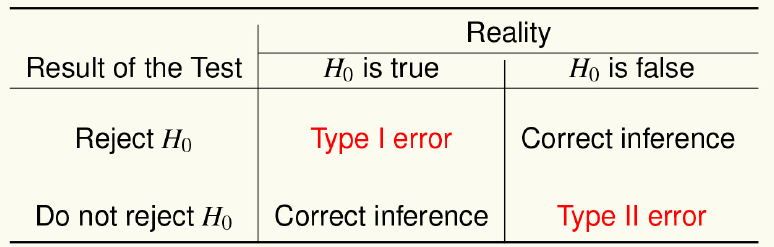
\includegraphics[width=\textwidth]{typeI_II_errors.png}
	\caption{Type I and Type II Errors}
\end{figure}

\section{Distributions}

\subsection{Discrete Distributions}
\subsubsection{Bernoulli Distribution}
A Bernoulli random variable $X$ is either zero or one.
\[
\mathbb{P}(X = 0) = p,  \mathbb{P}(X = 1) = 1-p 
\]

PMF and CDF:
\[
        \mathbb{P}(X=x) = p^x(1-p)^{1-x}
\]
\[
        F(x) = \begin{cases}
            0& x<0\\
            p& 0 \leq x\leq 1\\
            1& x >1
            \end{cases}     
\]

Mean and variance of Bernoulli distribution:
\[
    \begin{aligned}
        \mu &= p\\
        \sigma^2 &= p(1-p)       
    \end{aligned}
\]



\subsubsection{Binomial Distribution}
PMF and CDF:
\[
    \mathbb{P}(n;N,p) = \binom N n p^n(1-p)^{N-n}
\]
\[
    F(k;N,p) = \mathbb{P}(X\leq k) = \sum_{i=0}^{|k|} \binom N i p^i(1-p)^{N-i}
\]

Mean and variance:
\[
    \begin{aligned}
        \mu &= Np\\
        Var(X) &= Np(1-p)
    \end{aligned}
\]

\subsubsection{Poisson Distribution}
\[
    \mathbb{P}(X=n) = \frac{\lambda^n}{n!}e^{-\lambda}
\]

Mean and variance:
\[
    \begin{aligned}
        \mu &= \lambda\\
        Var(X) &= \lambda
    \end{aligned}
\]

\subsection{Continuous Distributions}

\subsubsection{Normal Distribution}
If $X \stackrel{d}{\sim} \mathcal{N}(\mu,\sigma^2)$, the PDF and CDF:
\[
f(x) = \frac{1}{\sqrt{2\pi \sigma^2}} \exp(-\frac{1}{2}(\frac{x-\mu}{\sigma})^2)
\]
\[
    F(x) = \frac{1}{2}(1+\mathrm{erf}(\frac{x-\mu}{\sigma \sqrt{2}}))
\]

Where erf denotes error function:
\[
    \mathrm{erf} z= \frac{2}{\sqrt{\pi}}\int_0^z e^{-t^2}dt 
\]

Mean and Variance:
\[
\begin{aligned}
    \mathbb{E}(x) &= \int_{-\infty}^{\infty}xf(x)dx = \mu\\
    \mathrm{Var}(x) &= \int_{-\infty}^{\infty}(x-\mu)^2 f(x)dx = \sigma^2
\end{aligned}    
\]

\subsubsection{Lognormal Distribution}
If $Y \sim \mathcal{N}(\mu,\sigma)$, we define $X = e^Y$, then we say X follows Lognormal Distribution.

PDF:
\[
    f(x) = \frac{1}{x\sigma \sqrt{2\pi}} \exp(-\frac{(\ln x-\mu)^2}{2\sigma^2})
\]

CDF:
\[
    F(x) = \frac{1}{2}(1+\mathrm{erf}(\frac{\ln x-\mu}{\sigma \sqrt{2}}))
\]

Mean and Variance:
\[
\begin{aligned}
    \mathbb{E}(x) &= \exp (\mu + \frac{\sigma^2}{2}) \\
    \mathrm{Var}(x) &= (\exp (\sigma^2)-1)\exp (2\mu + \sigma^2)
\end{aligned}    
\]

\subsubsection{Chi-Squared Distribution}
Suppose we have $k$ independent normal variables $z_1,\cdots,z_k$, let $S = \sum_{i=1}^k {z_i}^2$, then we say $S$ follows Chi-Squared Distribution:
\[
    S \sim \chi_k^2
\]

PDF:
\[
    f(x) = \frac{1}{2^{k/2}\Gamma(k/2)} x^{k/2 -1}e^{-x/2}
\]

Where $\Gamma$ function is defined:
\[
    \Gamma(n) = \int_0^\infty x^{n-1}e^{-x} dx
\]

% CDF:
% \[
%     F(x) = \frac{1}{\Gamma(k/2)}\mathrm{\gamma}(\frac{k}{2},\frac{x}{2})
% \]

Mean and Variance:
\[
\begin{aligned}
    \mathbb{E}(x) &= k \\
    \mathrm{Var}(x) &= 2k
\end{aligned}    
\]

\subsubsection{Student’s $t$ Distribution}
Let $Z \sim \mathcal{N}(0,1)$, $U \sim \chi_k^2$, we define:
\[
    X = \frac{Z}{\sqrt{U/k}}
\]

Then $X$ follows Student’s $t$ distribution:
\[
    X \sim t(K)
\]

PDF:
\[
    f(x) = \frac{\Gamma(\frac{k+1}{2})}{\sqrt{k\pi}\Gamma(\frac{k}{2})} (1+\frac{x^2}{k})^{-\frac{k+1}{2}}
\]

Mean and Variance:
\[
\begin{aligned}
    \mathbb{E}(x) &= 0 \\
    \mathrm{Var}(x) &= \frac{k}{k-2}
\end{aligned}    
\]

Note that t-distributed random variable will be the test statistic of sample mean esitimates.

\subsubsection{F-Distribution}
If $U_1 \sim \chi_{k_1}^2$, $U_2 \sim \chi_{k_2}^2$, $U_1$ and $U_2$ are independent, we define
\[
    X = \frac{U_1/k_1}{U_2/k_2}
\]

Then we say $X$ follows F-Distribution:
\[
    X \sim \mathrm{F}(k_1,k_2)
\]

PDF:
\[
    f(x) = \frac{
        \sqrt{
            \frac{(k_1x)^{k_1}k_2^{k_2}}{(k_1x+k_2)^{k_1+k_2}}
        }
    }{x \mathrm{B}(\frac{k_1}{2},\frac{k_2}{2})}
\]\
Where
\[
    \mathrm{B}(x,y) = \int_0^1 z^{x-1}(1-z)^{y-1}dz
\]

Mean and variance:
\[
    \begin{aligned}
        \mu &= \frac{k_2}{k_2-2}\\
        \sigma^2 &= \frac{2k_2^2(k_1+k_2-2)}{k_1(k_2-2)^2(k_2-4)}
    \end{aligned}
\]

F-distribution has properties:
\begin{itemize}
    \item When $k_1,k_2$ aprroximate infinity, F-distribution equals to standard normal distribution.
    \item If $X\sim t(k)$, then $X^2 \sim \mathrm{F}(1,k)$.
\end{itemize}
\section{Cross Sectional Estimation Frameworks}
\subsection{Ordinary Least Squares(OLS)}
\subsubsection{Simple OLS}

Model 0 is $Y_i = a+e_i$.

But given n pairs of observations on explanatory variable $X_i$ and dependent variable $Y_i$, we can have Model 1 by postulating that
\[
    Y_i = a + bX_i + e_i, \ i=1,2,\cdots,n,
\]
where $e_i$ is the noise.

Assumptions:
\begin{enumerate}
    \item $\mathbb{E}(e_i) = 0$ for every $i$
    \item $\mathbb{E}(e_i^2) = \sigma_e^2$
    \item $\mathbb{E}(e_i,e_j) = 0$ for every $i,j$
    \item $X_i,e_j$ are independednt for each $i,j$
    \item $e_i\sim \mathcal{N}(0,\sigma_e^2)$
\end{enumerate}

Least Sqaures: Minimizing the sum of squared errors:
\[
     \min_{\hat{a},\hat{b}}\sum_{i=1}^n e_i^2 = \sum_{i=1}^n(Y_i-\hat{a}-\hat{b}X_i)^2
\]

Set the first derivative of $a$ and $b$ as 0, we get:
\[
    \begin{aligned}
        \hat{a} &= \bar{Y} - \hat{b}\bar{X}\\
        \hat{b} &= \frac{\sum_{i=1}^nX_i(Y_i-\bar{Y})}{\sum_{i=1}^nX_i(X_i-\bar{X})}    \\
        &=\frac{\sum_{i=1}^n(X_i-\bar{X})(Y_i-\bar{Y})}{\sum_{i=1}^n(X_i-\bar{X})(X_i-\bar{X})}\\
        &=\frac{\mathbb{C}(Y,X)}{\mathbb{V}(X)}
    \end{aligned}
\] 

Properties of $\hat{a},\hat{b}$:

\[
    \begin{aligned}
        \hat{a} &\sim \mathcal{N}\left(a,\sigma_e^2\left(\frac{1}{n}+\frac{\bar{X}^2}{\sum_{i=1}^n\left(X_i-\bar{X}\right)^2}\right)\right)\\
        \hat{b} &\sim \mathcal{N}\left(b,\sigma_e^2\left(\frac{1}{\sum_{i=1}^n\left(X_i-\bar{X}\right)^2}\right)\right)
    \end{aligned}
\]
\begin{note}
    Because $\mathbb{E}(\hat{a}) = a$ ,$\mathbb{E}(\hat{b}) = b$, the $\hat{a}, \hat{b}$ are unbiased. Then Gauss-Markov Theorem states $\hat{a}$ and $\hat{b}$ has smallest variances, so $\hat{a}$ and $\hat{b}$ are efficient.
\end{note}

\subsubsection{Gauss-Markov Theorem}

\begin{theorem}{Gauss-Markov Theorem}
    states that among all linear and unbiased estimators, the OLS estimators $\hat{a}$ andb $\hat{b}$ have the minimum variances.
\end{theorem}

\subsubsection{OLS in Matrix}
Write model as $\mathbf{y} = \mathbf{X}\beta + \mathbf{e}$, by calculation, we get:
\[
    \hat{\beta} = (\mathbf{X}^{\prime}\mathbf{X})^{-1}\mathbf{X}^{\prime}\mathbf{y}
\]

\subsubsection{Hypothesis Testing}
Series of residuals:
\[
    \hat{e_i} = Y_i - \hat{a} - \hat{b}X_i, \ i=1,2,\cdots,n
\]

Testing null hypothesis $H_0: b =\beta (e.g.\ \beta = 0)$:
\[
    t_{n-2} = \frac{\hat{b}-\beta}{\hat{\sigma^e}\sqrt{\frac{1}{\sum_{i=1}^n(X_i-\bar{X})^2}}}
\]

Testing null hypothesis $H_0: a =\alpha (e.g.\ \alpha = 0)$:
\[
    t_{n-2} = \frac{\hat{a}-\alpha}{\hat{\sigma^e}\sqrt{\frac{1}{n}+\frac{\bar{X}^2}{\sum_{i=1}^n(X_i-\bar{X})^2}}}
\]

\begin{note}
    The denominators in testings are \textbf{standard errors} of $\hat{b}$ and $\hat{a}$.
\end{note}

\subsubsection{Consistent Properties of OLS}
\begin{enumerate}
    \item OLS $\hat{b}$ estimator is consistent: \[\lim_{n \to \infty} \hat{b} = b\]
    \item OLS $\hat{a}$ estimator is consistent: \[\lim_{n \to \infty} \hat{a} = a\]
\end{enumerate}

\subsubsection{Decomposition}
\begin{itemize}
    \item TSS: Total Sum of Squares
    \item ESS: Explained Sum of Squares
    \item RSS: Residual Sum of Squares
\end{itemize}

\[
    \begin{aligned}
        \mathrm{TSS} &= \sum_{i=1}^n(Y_i-\bar{Y})^2\\
        \mathrm{ESS} &= \sum_{i=1}^n(\hat{Y_i}-\bar{Y})^2\\
        \mathrm{RSS} &= \sum_{i=1}^n\hat{e_i}^2 = \sum_{i=1}^n(Y_i-\hat{Y})^2\\
        \mathrm{TSS} &= \mathrm{ESS} + \mathrm{RSS}\\
        R^2 &\coloneqq \frac{ESS}{TSS}
    \end{aligned}
\]

\subsubsection{Point Forecast and Confidence Interval}
The point forecast is 
\[
    \hat{Y_{n+1}} = \hat{a} + \hat{b}X_{n+1}
\]

With 95\% probability, the forecast value falls within the confidence interval bounded by
\[
    \hat{Y}_{n+1} \pm t_{n-2,97.5\%} \times \hat{\sigma_e}\sqrt{1+\frac{1}{n}+\frac{(X_{n+1}-\bar{X})^2}{\sum_{i=1}^n(X_i-\bar{X})^2}}
\]

\subsection{Discrete dependent variables}
\begin{itemize}
    \item Probit/logit model: used for binary dependent variables
    \item Multinomial probit/logit: Categorical dependent variables
    \item Ordered probit/logit: Discrete dependent variables
\end{itemize}

Probit:
\[
    \phi(X) = \mathbb{P}(Z\leq X) = \frac{1}{\sqrt{2\pi}}\int_{-\infty}^X \exp(-\frac{u^2}{2})du
\]

Logit:
\[
    \phi(X) = \mathbb{P}(Z\leq X) = \frac{1}{1+\exp(-k(X-X_0))}
\]

\begin{figure}[!ht]
	\centering
	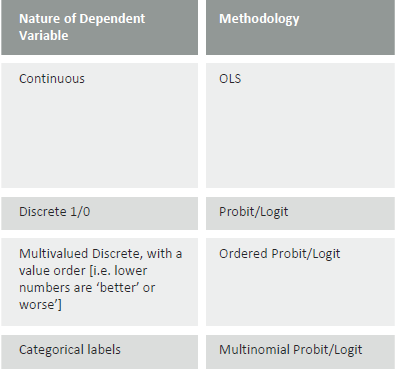
\includegraphics[width=\textwidth]{variables_method.png}
	\caption{Methodology roadmap}
\end{figure}

\section{Cross Sectional Estimation Techniques}
\subsection{Some notes}
\begin{figure}[!ht]
	\centering
	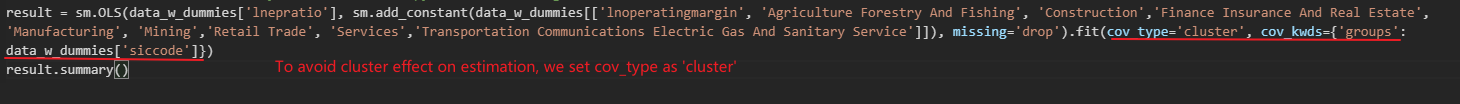
\includegraphics[width=\textwidth]{5/cluster.png}
\end{figure}
\begin{figure}[!ht]
	\centering
	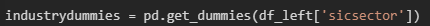
\includegraphics[width=\textwidth]{5/get_dummies.png}
\end{figure}
\begin{figure}[!ht]
	\centering
	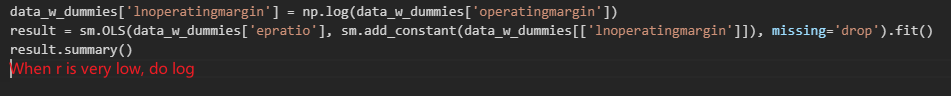
\includegraphics[width=\textwidth]{5/log.png}
\end{figure}
\begin{figure}[!ht]
	\centering
	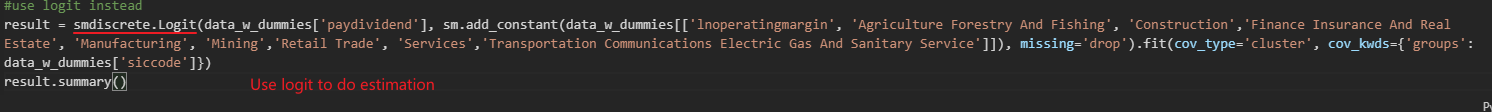
\includegraphics[width=\textwidth]{5/Logit.png}
\end{figure}
\begin{figure}[!ht]
	\centering
	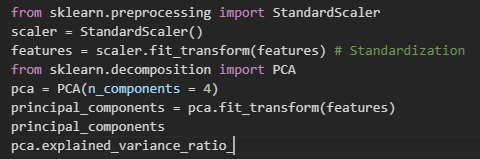
\includegraphics[width=\textwidth]{5/PCA.png}
\end{figure}

\begin{remark}
    Some key words: Fixed effects: dummy variables; t-statistic low: log; intra-cluster correlations: clustering; Collinearity: PCA; adding squared term; Hazard model; survival analysis 
\end{remark}
\section{CAPM (Cross Sectional Application), and Tests}
\subsection{Capital Market Line(CML)}
\[
  \mathrm{Sharpe\ Ratio = \frac{\mathbb{E}(r_i-r_f)}{\sigma_i}}
\]
\subsection{Security Market Line(SML)}
\[
  r_i -r_f= \beta_i(r_m-r_f) 
\]

\[
  \mathrm{Treynor\ Ratio = \frac{r_i-r_f}{\beta_i}} = \frac{r_m-r_f}{1}
\]

\begin{figure}
  \centering
  \begin{minipage}[t]{.5\textwidth}   %%%% [t] here
  \centering
  \begin{tikzpicture}
    \draw[->](0,0)--(5,0) node[right,scale = 1]{{$\sigma_w$}};
    \draw[->](0,0)--(0,5) node[above,scale = 1]{$r_w$};
    \draw[->](0,1)--(4,5) node[above right,scale = 1]{\textcolor{orange}{CML}};
    \node [left,scale = 1] at (0,3) {$r_m$};
    \node [left,scale = 1] at (0,1) {$r_f$};
    \node [below,scale = 1] at (2,0) {$\sigma_m$};
    \draw[dashed](2,0)--(2,3);
    \draw[dashed](0,3)--(2,3);
  \end{tikzpicture}
  \captionof{figure}{CML}
  \label{fig:square}
\end{minipage}%
  \begin{minipage}[t]{.5\textwidth}   %%%% [t] here
      \centering
      \begin{tikzpicture}
        \draw[->](0,0)--(5,0) node[right,scale = 1]{{$\beta$}};
        \draw[->](0,0)--(0,5) node[above,scale = 1]{$r$};
        \draw[->](0,1)--(4,5) node[above right,scale = 1]{\textcolor{orange}{SML}};
        \node [left,scale = 1] at (0,3) {$r_m$};
        \node [left,scale = 1] at (0,1) {$r_f$};
        \node [below,scale = 1] at (2,0) {$1$};
        \draw[dashed](2,0)--(2,3);
        \draw[dashed](0,3)--(2,3);
      \end{tikzpicture}
      \captionof{figure}{SML}
      \label{fig:rect}
  \end{minipage}%
\end{figure}


\subsection{Market Model}
Market model assumes that any stock's log return $r_{it}$ is bivariate normally distriuted with $r_{mt}$.

A linear regression model of $r_{it}$ on $r_{mt}$ is 
\[
  r_{it} = a + br_{mt} + e_{it}
\]
where 
\[
  \begin{aligned}
    a &= \mathbb{E}(r_{it}) - \frac{\sigma_{im}}{\sigma_m^2}\mathbb{E}(r_{mt})\\
    b &= \frac{\sigma_{im}}{\sigma_m^2}
  \end{aligned}
\]
\begin{remark}
  In QF600, the we do regression on simple returns, not log returns. I do not know if both methods work fine or only exists one right version. 
\end{remark}
\subsection{Capital Asset Pricing Model(CAPM)}
CAPM:
\[
  \mathbb{E}(r_{it}-r_{ft}) = b_i\mathbb{E}(r_{mt}-r_{ft})
\]

Do regression:
\[
  r_{it} - r_{ft} = a_i + b_i(r_{mt}-r_{ft}) + e_{it}
\]

OLS estimation of beta:
\[
  \hat{b_i} = \frac{\sum_{t=1}^T(r_{mt}-\bar{r_m})(r_{it}-\bar{r_i})}{\sum_{t=1}^T(r_{mt}-\bar{r_m})^2}
\]

\subsubsection{Some measurements}
\begin{itemize}
  \item standard error of $a$:
    \[
      \hat{\sigma_e}\sqrt{\frac{1}{T}+\frac{\bar{X}^2}{\sum_{t=1}^T(X_t-\bar{X})^2}}
    \]
  \item standard error of $b$:
    \[
      \hat{\sigma_e}\sqrt{\frac{1}{\sum_{t=1}^T(X_t-\bar{X})^2}}
    \]
  \item sum squared resid/residual Sum of Squares(SSR/RSS):
  \[
    \mathrm{SSR/RSS} = \sum_{t=1}^T\hat{e_t}^2
  \]
  \item standard error of regression:
  \[
    \sigma_e = \sqrt{\frac{1}{T-2}\mathrm{SSR}}
  \]
  \item Treynor ratio:
  \[
    \mathrm{Treynor\ ratio} \defeq  r_{mt} - r_{ft} = \frac{r_{it}-r_{ft}}{\beta_i}
  \]
  \item Jensen's measure:
  \[
    \mathrm{Jensen's \ measure} \defeq \mathbb{E}(r_{it}-r_{ft}) - b_i\mathbb{E}(r_{mt}-r_{ft})
  \]
  \item Sharpe ratio:
  \[
    \mathrm{Shapre \ ratio} \defeq  \frac{\mathbb{E}(r_{it}-r_{ft})}{\sigma_i} 
  \]
  \item $M^2 measurement$:
  \[
    M^2 \defeq \E (r_{it}-r_{ft})\frac{\sigma_m}{\sigma_i} - \E (r_{mt}-r_{ft})
  \]
  \item Information ratio:
  \[
    \mathrm{Information\ ratio} \defeq \frac{\E (r_{it}-r_{ft})}{\sigma_{i-f}}
  \]
  \item active return:
  \[
    \mathrm{active\ return} \defeq r_{it} - r_{ft}
  \]
  \item tracking error/active risk:
  \[
    \mathrm{tracking\ error} \defeq \sigma_{i-f}
  \]
\end{itemize}

% \section{ElegantNote Instructions}
% \thispagestyle{empty}
% The brand new ElegantNote is redesigned on the basis of \LaTeX{} article, a more elegant note template! You can use either \hologo{pdfLaTeX} or \hologo{XeLaTeX} to compile\footnote{The test environment is Win10 + \TeX{} Live 2019.}. It is recommended that \hologo{pdfLaTeX} be used for notes in English while \hologo{XeLaTeX} be used for notes in Chinese.

% The new template has the following features:
% \begin{itemize}
%   \item two modes: good for eye mode (geye) and hazy mode;
%   \item different devices: Pad (default), Screen(beamer size), Kindle, PC (double-page) and normal (A4);
%   \item 5 color themes: \textcolor{eblue}{blue} (default),  \textcolor{egreen}{green}, \textcolor{ecyan}{cyan}, \textcolor{sakura}{sakura} and \textcolor{black}{black};
%   \item languages support: Chinese (default), English;
%   \item support \hologo{pdfLaTeX} and \hologo{XeLaTeX};
%   \item prettier captions, list environments, and unified fonts;
%   \item custmized global font size: 8pt, 9pt, 10pt, 11pt, 12pt, 14pt, 17pt and 20pt.
% \end{itemize}


% \subsection{Optional Modes}

% This template provides optional modes: good for eye mode (geye) and hazy mode, while the paper color is green for the former and light blue for the latter. you can use the following code to activate the desired mode:
% \begin{lstlisting}[frame=none]  
%   \documentclass[geye]{elegantnote} % or
%   \documentclass[mode=geye]{elegantnote}
%   \documentclass[hazy]{elegantnote} % or
%   \documentclass[mode=hazy]{elegantnote}
% \end{lstlisting}

% \begin{remark}
%   If you are expected to customize background, use:
%   \begin{lstlisting}
%     \definecolor{geyecolor}{RGB}{199,237,204}
%     \pagecolor{geyecolor}
%   \end{lstlisting}
% \end{remark}


% \subsection{Device Options}

% To make the notes more comfortable to read, we designed four output options (of different sizes) that correspond to different reading devices: Pad (default), Kindle, PC and A4paper. 

% \textcolor{red}{New}: For the convenience of notes presentation, version 2.20 offers a new option for device, i.e. \lstinline{device=screen}, which is similar to the size of MS Powerpoint with ratio aspect of 4:3 (2019/12/06).

% The options of output for different devices are
% \begin{lstlisting}[frame=none]  
%   \documentclass[device=pad]{elegantnote}    % ipad screen size
%   \documentclass[device=kindle]{elegantnote} % kindle screen size
%   \documentclass[device=pc]{elegantnote}     % double pages for pc 
%   \documentclass[device=normal]{elegantnote} % a4 normal page
%   \documentclass[device=screen]{elegantnote} % 4:3 PPT size
% \end{lstlisting}

% \begin{note}
% You can also select the device by using a direct assignment method, such as:
% \end{note}

% \begin{lstlisting}[frame=none]  
%   \documentclass[pad]{elegantnote}
%   \documentclass[kindle]{elegantnote}
%   \documentclass[pc]{elegantnote}
%   \documentclass[normal]{elegantnote}
%   \documentclass[screen]{elegantnote}
% \end{lstlisting}

% \begin{note}
% To get a normal A4paper size PDF, please select \lstinline{device=normal}.
% \end{note}

% \subsection[Color Themes]{Color Themes\footnote{Test for chapter footnote.}}

% This template contains 5 color themes, \textcolor{egreen}{green}, \textcolor{ecyan}{cyan}, \textcolor{eblue}{blue}(default), \textcolor{sakura}{sakura} and \textcolor{black}{black}. If you don't need color, you can choose black theme. The color theme is enabled in the same way as before:
% \begin{lstlisting}[frame=none]  
%   \documentclass[green]{elegantnote}
%   \documentclass[color=green]{elegantnote}
%   ....
%   \documentclass[black]{elegantnote}
%   \documentclass[color=black]{elegantnote}
% \end{lstlisting}


% \subsection{Languages}

% This template contains two sets of language environments, changing the language environment will change the title of table/figure (figure, table), article structure words (such as the table of contents, references, etc.), and the environment Introductory words (such as Theorem, Lemma, etc.). The different language modes are enabled as follows:
% \begin{lstlisting}[frame=none]  
%   \documentclass[cn]{elegantnote}
%   \documentclass[lang=cn]{elegantnote}
%   \documentclass[en]{elegantnote}
%   \documentclass[lang=en]{elegantnote}
% \end{lstlisting}

% \begin{note}
% Chinese characters are allowed in Chinese mode only. To type in Chinese characters in English mode, please include \lstinline{ctex}\footnote{Please use \lstinline{scheme=plain} to retain headlines in English.} or \lstinline{xeCJK} package.
% \end{note}


% \subsection{Theorem Class Environments}

% This template used the \lstinline{amsthm} to create theorems, there are 4 types of theorem environments
% \begin{itemize}
%   \item \textbf{Theorem-Class}: theorem, lemma, proposition, corollary;
%   \item \textbf{Definition-Class}: definition, conjecture, example;
%   \item \textbf{Remark-Class}: remark, note, case;
%   \item \textbf{Proof-Class}: proof.
% \end{itemize}

% \begin{remark}
% With the option \lstinline{lang=cn} , the introductory words of the theorem class environments will be changed to Chinese.
% \end{remark}


% \section{Writing Sample}

% We will define the integral of a measurable function in three steps. First, we define the integral of a nonnegative simple function. Let $E$ be the measurable set in $\mathcal{R}^N$.

% % source: https://www.maths.tcd.ie/~dwilkins/LaTeXPrimer/Theorems.html

% \begin{definition}[Left Coset]
% Let $H$ be a subgroup of a group~$G$.  A \emph{left coset} of $H$ in $G$ is a subset of $G$ that is of the form $xH$, where $x \in G$ and $xH = \{ xh : h \in H \}$. Similarly a \emph{right coset} of $H$ in $G$ is a subset of $G$ that is of the form $Hx$, where $Hx = \{ hx : h \in H \}$
% \end{definition}

% Note that a subgroup~$H$ of a group $G$ is itself a left coset of $H$ in $G$.

% \begin{lemma}[Size Of Left Coset]
% Let $H$ be a finite subgroup of a group $G$.  Then each left
% coset of $H$ in $G$ has the same number of elements as $H$.
% \end{lemma}

% \begin{theorem}[Lagrange's Theorem]
% Let $G$ be a finite group, and let $H$ be a subgroup
% of $G$.  Then the order of $H$ divides the order of $G$.
% \end{theorem}

% \begin{proof}
% Let $z$ be some element of $xH \cap yH$.  Then $z = xa$ for some $a \in H$, and $z = yb$ for some $b \in H$. If $h$ is any element of $H$ then $ah \in H$ and $a^{-1}h \in H$, since $H$ is a subgroup of $G$. But $zh = x(ah)$ and $xh = z(a^{-1}h)$ for all $h \in H$. Therefore $zH \subset xH$ and $xH \subset zH$, and thus $xH = zH$.  Similarly $yH = zH$, and thus $xH = yH$, as required.
% \end{proof}

% \begin{figure}[!htbp]
% 	\centering
% 	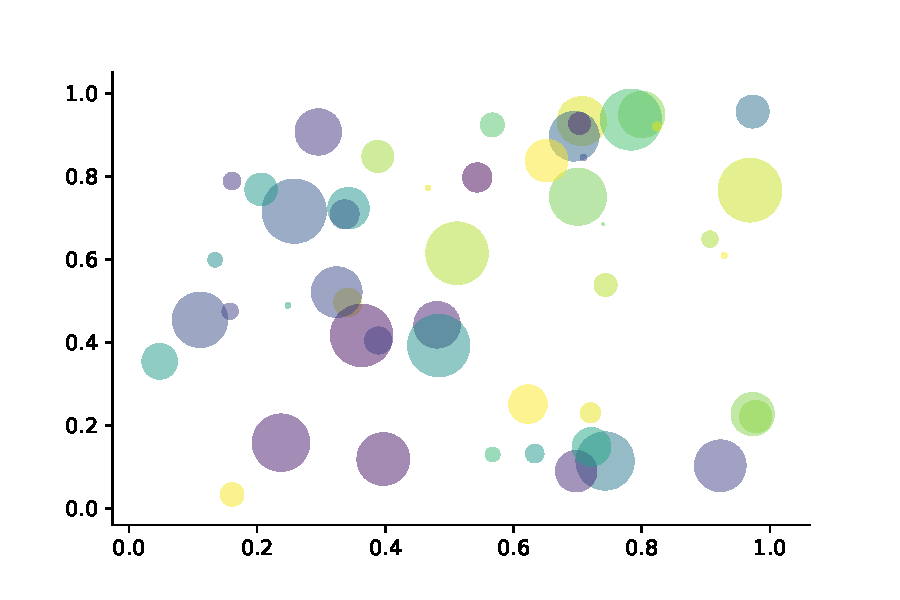
\includegraphics[width=0.6\textwidth]{scatter.pdf}
% 	\caption{Matplotlib: Scatter Plot Example\label{fig:mpg}}
% \end{figure}

% Regression analysis is a powerful statistical method that allows you to examine the relationship between two or more variables of interest. While there are many types of regression analysis, at their core they all examine the influence of one or more independent variables on a dependent variable. The process of performing a regression allows you to confidently determine which factors matter most, which factors can be ignored, and how these factors influence each other.

% Let's continue using our application training example. In this case, we'd want to measure the historical levels of satisfaction with the events from the past three years or so, as well as any information possible in regards to the independent variables. 

% \begin{table}[htbp]
%   \small
%   \centering
%   \caption{Auto MPG and Price \label{tab:reg}}
%     \begin{tabular}{lcc}
%     \toprule
%                     &       (1)         &        (2)      \\
%     \midrule
%     mpg             &    -238.90***     &      -49.51     \\
%                     &     (53.08)       &      (86.16)    \\
%     weight          &                   &      1.75***    \\
%                     &                   &      (0.641)    \\
%     constant        &     11,253***     &       1,946     \\
%                     &     (1,171)       &      (3,597)   \\
%     obs             &        74         &         74     \\
%     $R^2$           &      0.220        &       0.293    \\
%     \bottomrule
%     \multicolumn{3}{l}{\scriptsize Standard errors in parentheses} \\
%     \multicolumn{3}{l}{\scriptsize *** p<0.01, ** p<0.05, * p<0.1} \\
%     \end{tabular}%
% \end{table}%


% \begin{itemize}[noitemsep]
%   \item Routing and resource discovery;
%     \begin{itemize} 
%       \item Language Models
%       \item Vector Space Models
%     \end{itemize}
%   \item Resilient and scalable computer networks;
%   \item Distributed storage and search.
% \end{itemize}


% \section{Recruit Support Members}

% Recruit support members for Elegant\LaTeX{} to translate template official guide, maintain wiki entries, update Wechat articles. No deadline for this recruitment.

% So far, Elegant\LaTeX{} has four support members:
% \begin{itemize}
% 	\item OG Translator: \href{https://github.com/peggy2006xzyz}{YPY};
% 	\item Wiki Maintainer: \href{https://github.com/izinngo}{Ingo Zinngo}, \href{https://github.com/xiaohao890809}{Xiaohao890809};
% 	\item QQ Group Manager: \href{https://github.com/sikouhjw}{Sikouhjw}.
% \end{itemize}

% Thank them all!!!

% \section{Acknowledgement}
% The number of stars on Github for ElegantPaper reached 176 on Dec. 8, 2019 at the release of ElegantNote v2.40.
% Thank China\TeX{} and \href{http://www.latexstudio.net/}{\LaTeX{} studio} for their promotion. 

% If you like our templates, star on Github.
% \begin{figure}[!ht]
% 	\centering
% 	\includegraphics[width=\textwidth]{star.png}
% 	\caption{Twinkle, Twinkle, Little Star}
% \end{figure}

% \section{Donation}
% To express your love for our templates and/or our developers, please do not hesitate to tip us.
% \begin{figure}[!htbp]
% 	\centering
% 	
\includegraphics[width=0.4\textwidth]{donate.jpg}
% \end{figure}

% \textbf{The explanation right of the tip usage belongs to Elegant\LaTeX{} with no supervision. Feel free to tip us.} Those who donate more than 10 RMB will be recorded in the donation list and will receive a donation certificate. Thank all the tippers!

% \begin{table}[htbp]
%   \centering
%   \caption{Donation List}
%     \begin{tabular}{cccccccc}
%     \toprule
%     \textbf{Tipper} & \textbf{Amount} & \textbf{Date} & \textbf{Channel} & \textbf{Tipper} & \textbf{Amount} & \textbf{Date} & \textbf{Channel} \\
%     \midrule
%     Lerh  & 10 RMB & 2019/5/15 & Wechat & LIU ZhiKuo & 100 RMB & 2019/10/15 & Alipay \\
%     DiPingXian & 10 RMB & 2019/5/15 & Wechat & * Tao & 16 RMB & 2019/10/17 & Wechat \\
%     YinSang & 20 RMB & 2019/5/27 & Wechat & ChiHong & 12 RMB & 2019/10/17 & Alipay \\
%     * Kong & 10 RMB & 2019/5/30 & Wechat & YuanFengJing & 10 RMB & 2019/10/28 & Wechat \\
%     latexstudio.net & 666 RMB & 2019/6/05 & Alipay & GUO DeLiang & 88 RMB & 2019/11/03 & Wechat \\
%     Cassis & 11 RMB & 2019/6/30 & Wechat & ZiQiangBuXi & 20 RMB & 2019/11/03 & Alipay \\
%     * Jun & 10 RMB & 2019/7/23 & Wechat & DuShuZhiChong & 20 RMB & 2019/11/18 & Wechat \\
%     P*u   & 50 RMB & 2019/7/30 & Wechat & * Deng & 10 RMB & 2019/11/18 & Wechat \\
%     * Meng & 19 RMB & 2019/8/28 & Wechat & * Zhe & 20 RMB & 2019/11/18 & Wechat \\
%     QuDouDou & 10 RMB & 2019/8/28 & Wechat & anonymous & 10 RMB & 2019/11/24 & Wechat \\
%     LI Bo & 100 RMB & 2019/10/06 & Wechat & Jiye Qian & 66 RMB & 2019/12/04 & Wechat \\
%     Njustsll & 10 RMB & 2019/10/11 & Wechat & Boy Yang & 20 RMB & 2019/12/05 & Wechat \\
% \bottomrule
% \end{tabular}%
%   \label{tab:donation}%
% \end{table}%


% \section{FAQ}

% \begin{enumerate}[label=\arabic*).]
% 	\item \textit{How to remove the information of version?}\\
%     Please comment \lstinline|\version{x.xx}|.
% 	\item \textit{How to remove the information of date?}\\
% 	  Please type in \lstinline|\date{}|.
% 	\item \textit{How to add several authors?}\\
% 	  Use \lstinline{\and} in \lstinline{\author} and use \lstinline{\\} to start a new line.
%     \begin{lstlisting}
%       \author{author 1\\ org. 1 \and author 2 \\ org. 2 }
%     \end{lstlisting}
% \end{enumerate}

% \section{A Minimal Example}

% \begin{lstlisting}
% \documentclass[en,hazy,blue,screen,14pt]{elegantnote}

% \title{ElegantNote Example}
% \author{ddswhu}
% \institute{Elegant\LaTeX{} Program}
% % \version{1.00}
% \date{}

% \begin{document}

% \maketitle

% \section{Introduction}

% The content of Introduction.

% \end{document}
% \end{lstlisting}

\end{document}
